\documentclass[../notes.tex]{subfiles}

\pagestyle{main}
\renewcommand{\chaptermark}[1]{\markboth{\chaptername\ \thechapter\ (#1)}{}}
\setcounter{chapter}{4}

\begin{document}




\chapter{Misc. Reactive Intermediates}
\section{Radicals}
\begin{itemize}
    \item \marginnote{10/1:}Lecture 7 recap.
    \begin{itemize}
        \item Anion formation: \ce{R-H <=> R- + H+}.
        \item $\pKa$'s are a measure of anion stability.
        \item Anions are stabilized by\dots
        \begin{itemize}
            \item Electronegative substituents (that withdraw electron density);
            \item More $s$-character (to hold the negative charge closer to the positive nucleus);
            \item Delocalization/resonance (to spread out the negative charge);
            \item Orbital overlap with adjacent atoms (along the lines of reverse hyperconjugation, e.g., in the case of ylides).
        \end{itemize}
        \item Anions are pyramids with low inversion barriers, and hence are effectively planar.
    \end{itemize}
    \item Today: Radicals.
    \item Lecture outline.
    \begin{itemize}
        \item Structure of radicals.
        \item Stability of radicals (thermodynamic and kinetic).
        \item Bond dissociation energy.
        \item Synthesis of radicals.
        \item Radical reactions.
        \item Probing radical mechanisms: Radical clocks, traps, and cages.
        \item Radical ions.
    \end{itemize}
    \item Structure of radicals.
    \begin{figure}[h!]
        \centering
        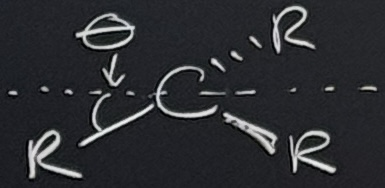
\includegraphics[width=0.12\linewidth]{anglePlanarity.JPG}
        \caption{Angle of deviation from planarity.}
        \label{fig:anglePlanarity}
    \end{figure}
    \begin{itemize}
        \item Most radicals are shallow pyramids with small inversion barriers ($<\SI[per-mode=symbol]{5}{\kilo\calorie\per\mole}$).
        \begin{itemize}
            \item The methyl radical (\ce{*CH3}) is planar by $\sim\SI[per-mode=symbol]{10}{\kilo\calorie\per\mole}$.
            \item Recall the discussion of its QMOT diagram (Figure \ref{fig:QmotCH3})!
        \end{itemize}
        \item As with anions, electronegative substituents raise the inversion barrier.
        \begin{itemize}
            \item For example, the trifluoromethyl radical (\ce{*CF3}) is pyramidal.
        \end{itemize}
        \item Increasing sterics favor pyramidalization (more $p$-character)?? Wouldn't bulky groups push apart?
        \item Consider the angle of deviation $\theta$ from planarity.
        \begin{itemize}
            \item The ethyl radical ($1^\circ$) has $\theta=\ang{11.9}$.
            \item The isopropyl radical ($2^\circ$) has $\theta=\ang{18.6}$.
            \item The isobutyl radical ($3^\circ$) has $\theta=\ang{24.1}$.
        \end{itemize}
    \end{itemize}
    \item Thermodynamic stability of radicals.
    \begin{itemize}
        \item Delocalization stabilizes radicals.
        \begin{itemize}
            \item Delocalization with neighboring heteroatoms is especially stabilizing!
        \end{itemize}
        \item Hyperconjugation stabilizes radicals.
        \begin{itemize}
            \item Thus, in terms of decreasing stability, $3^\circ>2^\circ>1^\circ$.
            \item This is analogous to cations.
        \end{itemize}
        \item More $p$-character stabilizes radicals.
        \begin{itemize}
            \item Thus, in terms of decreasing stability, $p>sp^3>sp^2>sp>s$.
            \item This is because radicals are inherently electron deficient, so they want to be further from the $\delta^+$ nucleus.
            \item This is the opposite of anions!
            \item Alternatively: The more $s$-character, the stronger the bond, and hence the less stable the radical formed by homolytic bond cleavage.
            \begin{itemize}
                \item We'll formalize this notion with \textbf{BDEs} in just a moment.
            \end{itemize}
        \end{itemize}
        \item More electronegative atoms destabilize the radical center.
        \begin{itemize}
            \item Thus, in terms of decreasing stability, $\ce{*C}>\ce{*N}>\ce{*O}$.
        \end{itemize}
        \item Larger atomic size stabilizes radicals.
        \begin{itemize}
            \item Thus, in terms of decreasing stability, $\ce{*S}>\ce{*O}$.
            \item This is because larger atoms are more polarizable.
        \end{itemize}
    \end{itemize}
    \item Kinetic stability of radicals.
    \begin{itemize}
        \item Consider a relatively stable radical, such as one that has some resonance stabilization. Suppose we add some steric blocking to it. This yields a \textbf{persistent radical}.
    \end{itemize}
    \item \textbf{Persistent radical}: A kinetically stable radical that may even be shelf-stable.
    \begin{itemize}
        \item These are not thermodynamically stable: It's still a radical, so it doesn't want to exist. But it just won't react with anything.
        \item Classic example: \textbf{TEMPO}.
        \item Persistent radicals are useful for radical traps and other experiments discussed later this lecture.
    \end{itemize}
    \item \textbf{(2,2,6,6-Tetramethylpiperidin-1-yl)oxyl}: A common persistent radical. \emph{Also known as} \textbf{TEMPO}. \emph{Structure}
    \begin{figure}[H]
        \centering
        \begin{subfigure}[b]{0.3\linewidth}
            \centering
            \footnotesize
            \chemfig[fixed length=false]{?(-[6,0.8])(-[:130,0.8])-[:20]-[:-50]-[:170]-[:-160,,,,ovbnd](-[6,0.8])(-[:174,0.8])-[:130]N?(-[:-170]\charge{180=\.}{O})}
            \caption{Structure.}
            \label{fig:TEMPOa}
        \end{subfigure}
        \begin{subfigure}[b]{0.3\linewidth}
            \centering
            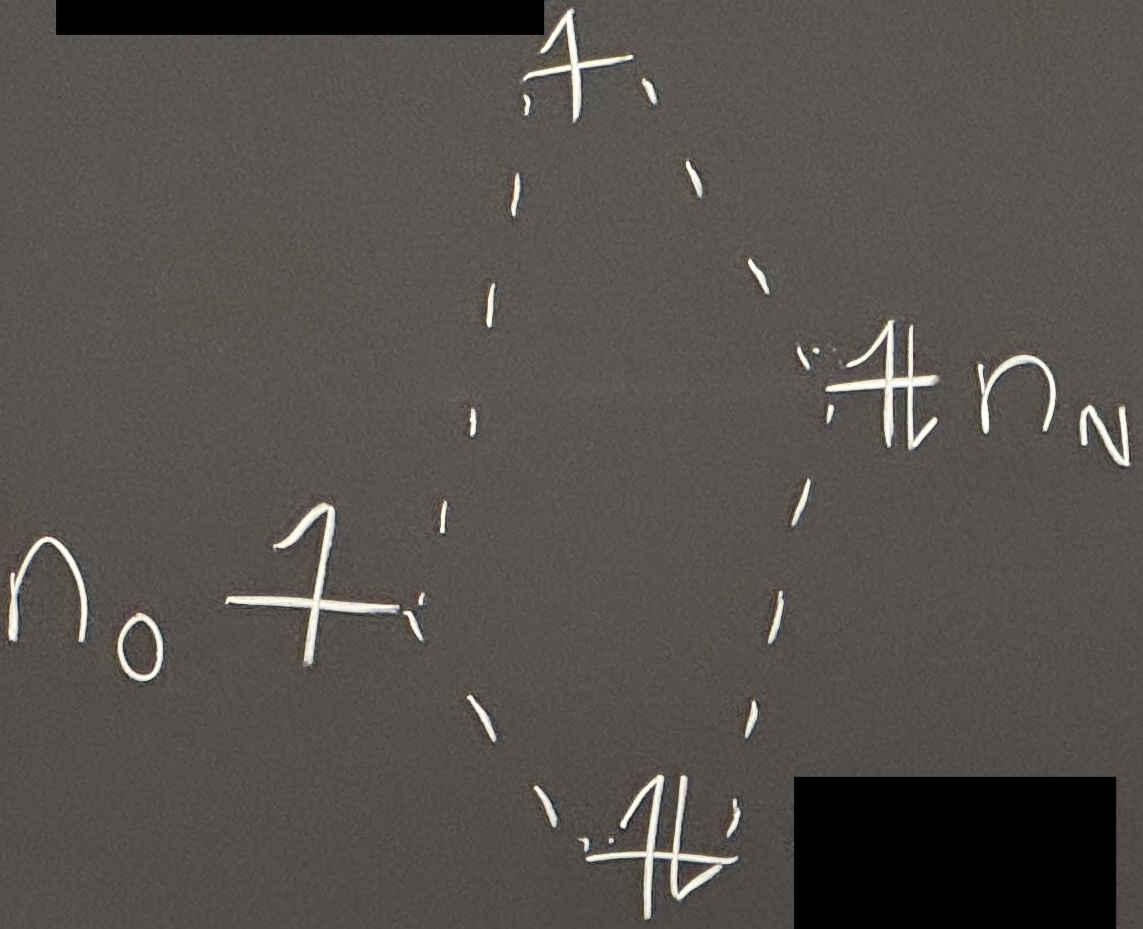
\includegraphics[width=0.6\linewidth]{TEMPOb.JPG}
            \caption{\ce{N-O*} molecular orbitals.}
            \label{fig:TEMPOb}
        \end{subfigure}
        \caption{TEMPO.}
        \label{fig:TEMPO}
    \end{figure}
    \begin{itemize}
        \item Formed by oxidizing 2,2,6,6-tetramethylpiperidine (TMP), a sterically hindered organic base, with \ce{H2O2} in the presence of the tungstate anion (\ce{WO4^2-}).
        \item Check: TEMPO \emph{does} have both resonance stabilization (with the adjacent nitrogen heteroatom) and steric blocking (from the adjacent quaternary carbons).
        \item The MO diagram (Figure \ref{fig:TEMPOb}) reveals that the \ce{N-O*} bond is an example of a 2c-3e bond.
        \item The \textbf{spin density map} shows that the radical is evenly dispersed on \ce{O} and \ce{N}: 50\% radical density on \ce{O} and 50\% on \ce{N}.
        \item Takeaway: If you want to design your own persistent radical, take something with some resonance, add some steric blockers, and you're good to go!
    \end{itemize}
    \item \textbf{Bond dissociation energy}: The energy it takes to symmetrically break a chemical bond. \emph{Also known as} \textbf{BDE}. \emph{Given by}
    \begin{equation*}
        \ce{X-Y <=> X* + Y*}\tag*{$\Delta H^\circ=\text{BDE}$}
    \end{equation*}
    \begin{itemize}
        \item Observe that this definition is analogous to those of HIA and $\pKa$ from the past two lectures!
        \item \ce{X} and \ce{Y} can be organic groups, hydrogen, heteroatoms, etc.
        \item The above reaction denotes \textbf{homolytic} bond cleavage, as opposed to \textbf{heterolytic}.
        \item BDE is an extremely useful measure of "bond strength." It's probably one of the top three key concepts we should take away from Phys Orgo to use in the rest of our careers.
        \begin{itemize}
            \item Guideline: A weak bond yields a more stable radical.
        \end{itemize}
        \item BDE is useful for predicting if a reaction is endothermic or exothermic.
        \item One big factor that affects BDE is bond polarity.
        \begin{itemize}
            \item In general, more polar bonds are stronger.
            \begin{itemize}
                \item This contrasts with heterolytic cleavage, where polar bonds are easier to cleave.
                \item Essentially, acidic bonds are "stronger" even if it's easier to take off the acidic proton with your own "hands" (reagents) in lab.
            \end{itemize}
            \item See Table \ref{tab:pKaBDE} for more.
            \item Key point: When we talk about "strong bonds," just remember that we're talking about the BDE.
        \end{itemize}
    \end{itemize}
    \item \textbf{Homolytic} (bond cleavage): The breaking of a chemical bond in such a way that an \emph{equal} amount of electron density is left on both products.
    \item \textbf{Heterolytic} (bond cleavage): The breaking of a chemical bond in such a way that an \emph{unequal} amount of electron density is left on both products.
    \item Let's look at some example comparisons between $\pKa$'s and BDE's to see the aforementioned inverse relationship.
    \begin{table}[h!]
        \centering
        \small
        \renewcommand{\arraystretch}{1.2}
        \begin{tabular}{l|cccc}
             & \textbf{\ce{H3C-H}} & \textbf{\ce{H2N-H}} & \textbf{\ce{HO-H}} & \textbf{\ce{F-H}}\\
            \hline
            \textbf{p\emph{K}\textsubscript{a} (\ce{H2O})} & 48 & 38 & 15.7 & 3.2\\
            \textbf{BDE (kcal/mol)} & 105 & 107 & 119 & 135\\
        \end{tabular}
        \caption{BDEs and $\pKa$'s are inversely related.}
        \label{tab:pKaBDE}
    \end{table}
    \begin{itemize}
        \item As we go to the right, it becomes easier to remove \ce{H+}.
        \item As we go to the left, it become easier to remove \ce{H*}.
    \end{itemize}
    \pagebreak
    \item Some BDEs to know. (Memorize these!! They will likely come up in your Quals!)
    \begin{itemize}
        \item The effect of bond polarity.
        \begin{itemize}
            \item \ce{C-C}: $\sim\SI[per-mode=symbol]{81}{\kilo\calorie\per\mole}$.
            \item \ce{C-H}: $\sim\SI[per-mode=symbol]{98}{\kilo\calorie\per\mole}$.
            \item \ce{O-H}: $\sim\SI[per-mode=symbol]{105}{\kilo\calorie\per\mole}$.
        \end{itemize}
        \item The effect of hyperconjugation.
        \begin{itemize}
            \item \ce{Me-H}: $\sim\SI[per-mode=symbol]{105}{\kilo\calorie\per\mole}$.
            \item \ce{Et-H}: $\sim\SI[per-mode=symbol]{100.5}{\kilo\calorie\per\mole}$.
            \item \ce{{}^{\emph{i}}Pr-H}: $\sim\SI[per-mode=symbol]{98.1}{\kilo\calorie\per\mole}$.
            \item \ce{{}^{\emph{t}}Bu-H}: $\sim\SI[per-mode=symbol]{95.7}{\kilo\calorie\per\mole}$.
        \end{itemize}
        \item The effect of hybridization.
        \begin{itemize}
            \item \ce{RC#C-H}: $\sim\SI[per-mode=symbol]{132.8}{\kilo\calorie\per\mole}$.
            \item \ce{R2C=CH-H}: $\sim\SI[per-mode=symbol]{111.2}{\kilo\calorie\per\mole}$.
            \item \ce{Ph-H}: $\sim\SI[per-mode=symbol]{112.9}{\kilo\calorie\per\mole}$.
        \end{itemize}
        \item The effect of resonance.
        \begin{itemize}
            \item \ce{All-H}: $\sim\SI[per-mode=symbol]{88.2}{\kilo\calorie\per\mole}$.
            \item \ce{Bn-H}: $\sim\SI[per-mode=symbol]{88.5}{\kilo\calorie\per\mole}$.
            \item Note that allyl bonds are broken more easily than benzyl ones because resonance stabilizing the product radical doesn't force you to break aromaticity; indeed, breaking aromaticity is a little less fun than moving a $\pi$-bond around.
        \end{itemize}
        \item The effect of atomic size and polarizability.
        \begin{itemize}
            \item \ce{Me-I}: $\sim\SI[per-mode=symbol]{57.1}{\kilo\calorie\per\mole}$.
            \item \ce{Me-Br}: $\sim\SI[per-mode=symbol]{70.3}{\kilo\calorie\per\mole}$.
            \item \ce{Me-Cl}: $\sim\SI[per-mode=symbol]{83.7}{\kilo\calorie\per\mole}$.
            \item \ce{Me-F}: $\sim\SI[per-mode=symbol]{110.0}{\kilo\calorie\per\mole}$.
        \end{itemize}
        \item Peroxides.
        \begin{itemize}
            \item \ce{HO-H}: $\sim\SI[per-mode=symbol]{119}{\kilo\calorie\per\mole}$.
            \item \ce{HO-OH}: $\sim\SI[per-mode=symbol]{51}{\kilo\calorie\per\mole}$.
            \item \ce{{}^{\emph{t}}BuOO-H}: $\sim\SI[per-mode=symbol]{88}{\kilo\calorie\per\mole}$.
            \item \ce{{}^{\emph{t}}BuO-OH}: $\sim\SI[per-mode=symbol]{44}{\kilo\calorie\per\mole}$.
            \item \ce{{}^{\emph{t}}BuO-H}: $\sim\SI[per-mode=symbol]{106}{\kilo\calorie\per\mole}$.
        \end{itemize}
    \end{itemize}
    \item Polar effects on radicals.
    \begin{figure}[h!]
        \centering
        \begin{subfigure}[b]{0.3\linewidth}
            \centering
            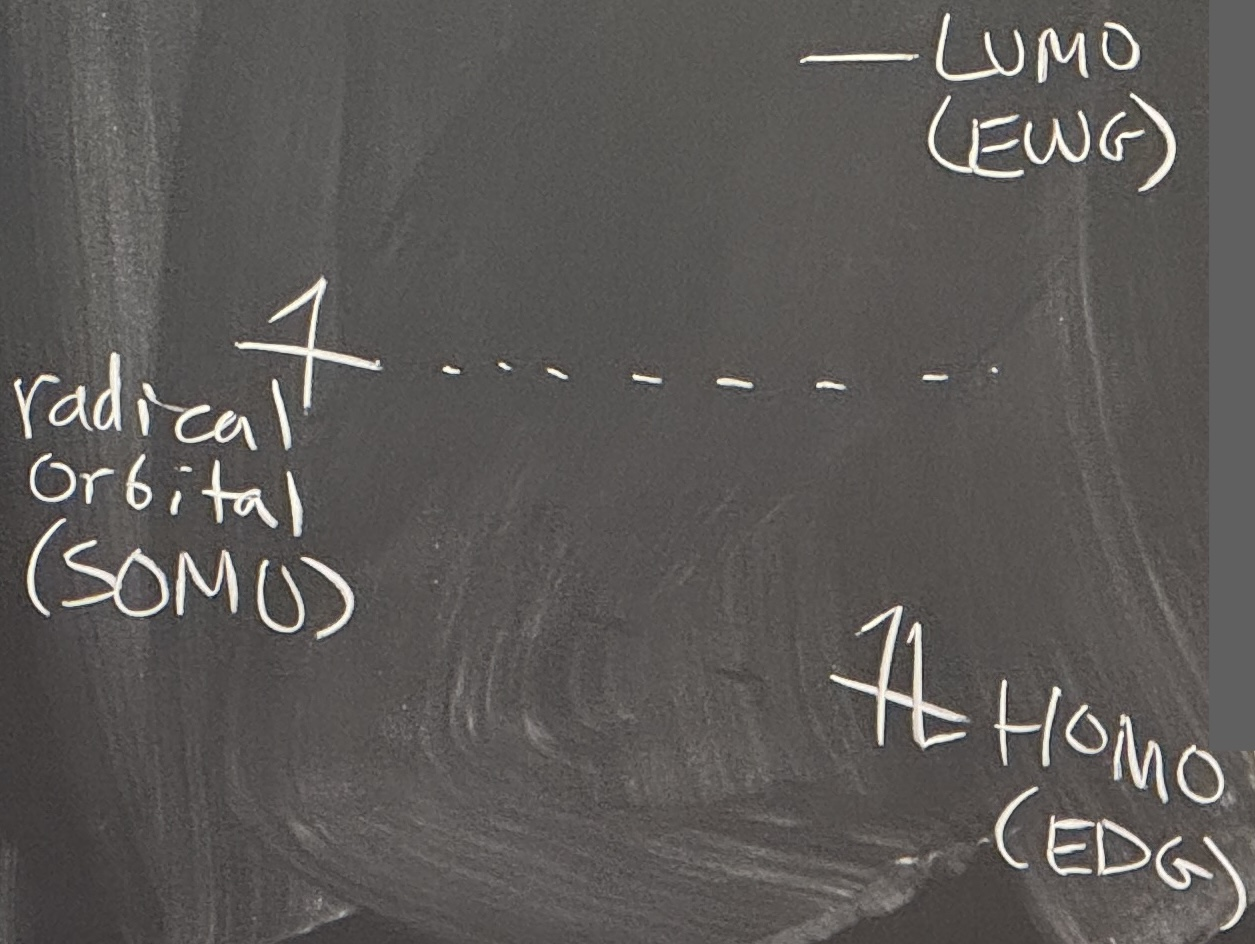
\includegraphics[width=0.83\linewidth]{polarRadicala.JPG}
            \caption{Unmixed radical energy.}
            \label{fig:polarRadicala}
        \end{subfigure}
        \begin{subfigure}[b]{0.3\linewidth}
            \centering
            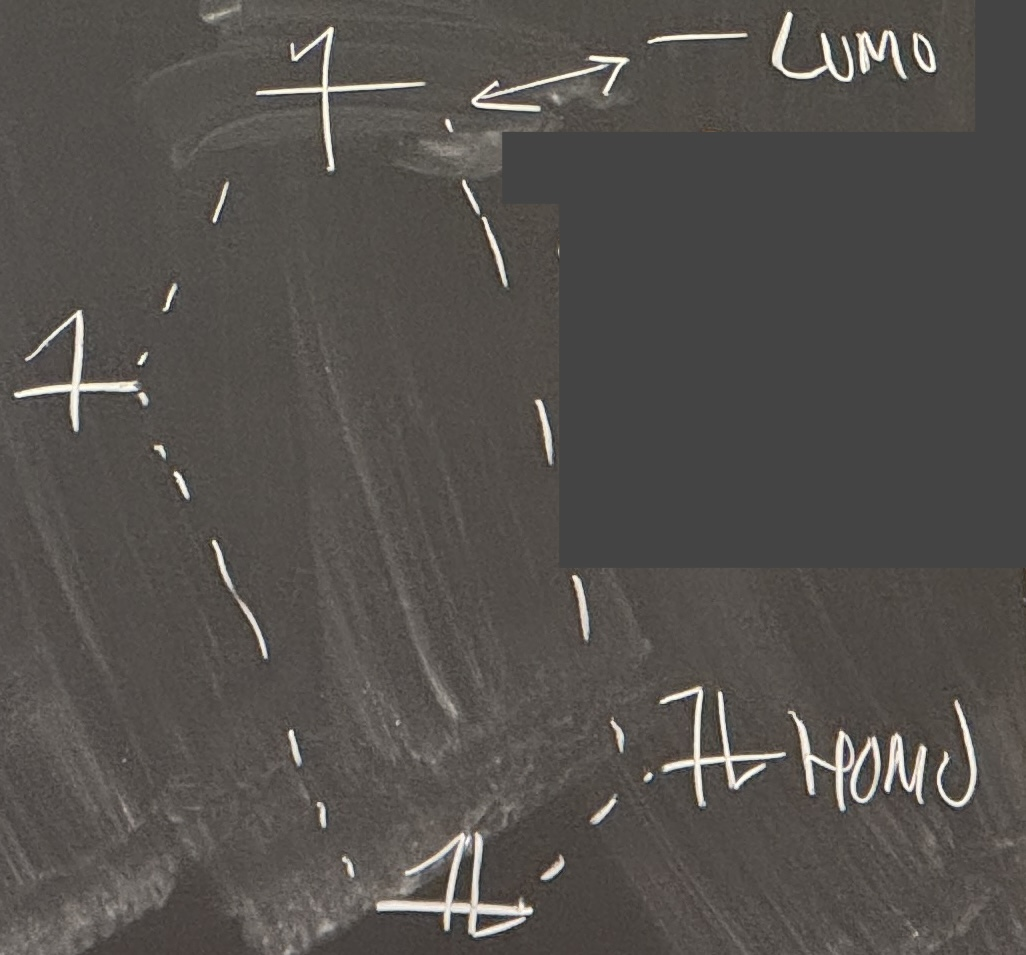
\includegraphics[width=0.75\linewidth]{polarRadicalb.JPG}
            \caption{Radical near EDG.}
            \label{fig:polarRadicalb}
        \end{subfigure}
        \begin{subfigure}[b]{0.3\linewidth}
            \centering
            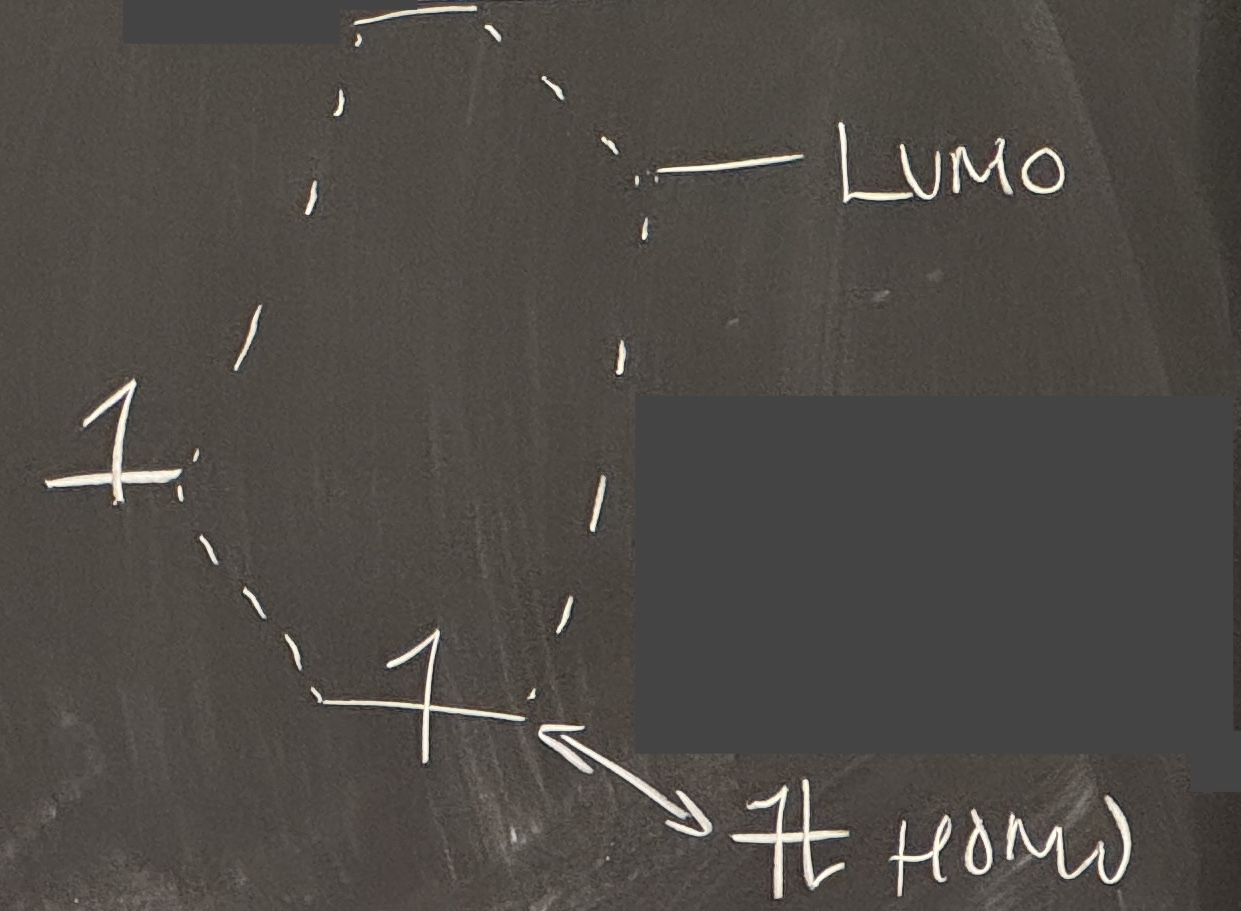
\includegraphics[width=0.8\linewidth]{polarRadicalc.JPG}
            \caption{Radical near EWG.}
            \label{fig:polarRadicalc}
        \end{subfigure}
        \caption{Radicals near EDGs and EWGs.}
        \label{fig:polarRadical}
    \end{figure}
    \pagebreak
    \begin{itemize}
        \item Both EDGs \emph{and} EWGs can stabilize radicals, despite the fact that radicals are electron deficient.
        \item Example: A radical $\alpha$ to a carbonyl (e.g., homolytically cleave one of acetone's \ce{C-H} bonds).
        \begin{itemize}
            \item The carbonyl \emph{will} destabilize the radical inductively.
            \item However, it will also \emph{stabilize} the radical through resonance.
            \item The second effect (resonance) is stronger.
        \end{itemize}
        \item Let's now justify these stabilizing effects using MO theory.
        \begin{itemize}
            \item Before mixing (Figure \ref{fig:polarRadicala}), a typical radical has energy intermediate between the HOMO of an EDG and the LUMO of an EWG.
            \item When a radical's SOMO interacts with the HOMO of an EDG (Figure \ref{fig:polarRadicalb}), \emph{two} electrons get stabilized and \emph{one} gets destabilized. It follows that there is a net stabilization of the molecule, as expected.
            \item When a radical's SOMO interacts with the LUMO of an EWG (Figure \ref{fig:polarRadicalc}), the sole electron present in the system gets stabilized. It follows that there is \emph{still} a net stabilization of the molecule, even here!
        \end{itemize}
        \item These molecular orbital diagrams reveal two additional attributes of polarized radicals, as well.
        \begin{enumerate}
            \item EDGs make radicals more nucleophilic.
            \begin{itemize}
                \item When a radical's SOMO interacts with the HOMO of an EDG (Figure \ref{fig:polarRadicalb}), a new radical SOMO (the antibonding orbital) is created.
                \item This new SOMO is a better energy match with LUMOs, so the radical electron is more likely to mix with a LUMO since this will lead to greater thermodynamic stabilization of the product than before.
                \item In other words, the radical is now more nucleophilic.
            \end{itemize}
            \item EWGs make radicals more electrophilic.
            \begin{itemize}
                \item When a radical's SOMO interacts with the LUMO of an EWG (Figure \ref{fig:polarRadicalc}), a new radical SOMO is once again created, but it is the stabilized bonding orbital this time.
                \item This new SOMO is a better energy match with HOMOs, so the radical electron is more likely to mix with a HOMO since this will lead to greater thermodynamic stabilization of the product than before.
                \item In other words, the radical is now more electrophilic.
            \end{itemize}
        \end{enumerate}
    \end{itemize}
    \item Synthesis of radicals.
    \begin{itemize}
        \item Also known as \textbf{initiation}, if we're doing a radical chain reaction.
        \item Most common way to make a radical: Homolytic cleavage of a weak bond.
        \begin{itemize}
            \item We'll often use light or heat to give a little burst of energy and break this bond.
        \end{itemize}
        \item Commonly used radical initiators.
        \begin{itemize}
            \item Peroxides are easily broken by light and heat, so we often use them.
            \begin{itemize}
                \item Example: Organic peroxides react like \ce{RO-OR ->[$h\nu$][$\Delta$] RO*}
            \end{itemize}
            \item \textbf{AIBN}.
            \item \ce{Br2}.
            \begin{itemize}
                \item Bromine reacts like \ce{Br-Br ->[$h\nu$][$\Delta$] Br*}
            \end{itemize}
            \item Paramagnetic metals, i.e., metals with 1 unpaired electron.
            \begin{itemize}
                \item Example: \textbf{\ce{Cp2Ti^{III}Cl}}.
            \end{itemize}
            \item Single-electron transfer (SET) or energy transfer (ET).
            \begin{itemize}
                \item Often done with metals, electrochemistry, or photochemistry.
                \item These are increasingly common ways to cycle one-electron oxidation states.
            \end{itemize}
        \end{itemize}
        \item Essentially, if we ever need to make a radical, we can choose old-school or new-school based on what we have on hand!
    \end{itemize}
    \item \textbf{Azobisisobutyronitrile}: A common thermal radical initiator. \emph{Also known as} \textbf{AIBN}.
    \begin{figure}[H]
        \centering
        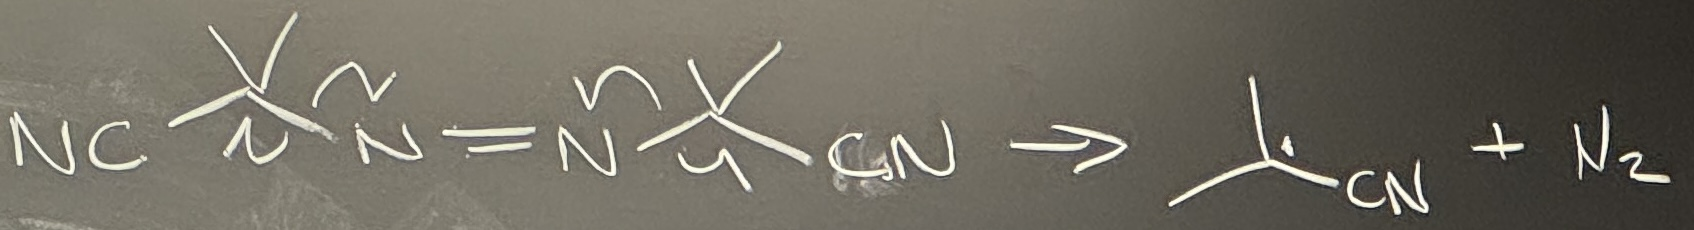
\includegraphics[width=0.45\linewidth]{AIBN.JPG}
        \caption{AIBN as a thermal radical initiator.}
        \label{fig:AIBN}
    \end{figure}
    \begin{itemize}
        \item This radical has a very cool design: Under heat or shock, you cleave the \ce{N-C} bonds to form tertiary radicals that are additionally stabilized by their proximity to a $\pi$-system, and release \ce{N2}.
        \item You commonly see AIBN used with \ce{HSnBu3} in radical cyclizations.
    \end{itemize}
    \item \textbf{Titanocene monochloride}: An increasingly popular SET agent. \emph{Denoted by} \textbf{\ce{Cp2Ti^{III}Cl}}.
    \begin{figure}[h!]
        \centering
        \footnotesize
        \schemestart
            \chemfig{*3([:-30]--O-)}
            \arrow{->[\ce{Cp2Ti^{III}Cl}]}[,1.6]
            \chemfig[atom sep=3em]{*4([4]Ti^{IV}-O--\charge{0=\.}{})}
            \arrow[,1.6]
            \chemfig{HO-[:-60]--[:60]H}
        \schemestop
        \caption{\ce{Cp2Ti^{III}Cl} as an SET radical initiator.}
        \label{fig:Cp2TiCl}
    \end{figure}
    \begin{itemize}
        \item For example, \ce{Cp2Ti^{III}Cl} can be used for radical-mediated epoxide openings, as shown above.
    \end{itemize}
    \item Radical reactions.
    \begin{figure}[h!]
        \centering
        \footnotesize
        \begin{subfigure}[b]{0.45\linewidth}
            \centering
            \schemestart
                \chemfig{\charge{0=\.}{R}}
                \+{1em}
                \chemfig{=_[:30]-[:-30]X}
                \arrow
                \chemfig{R-[:30]-[:-30]\charge{-90=\.}{}-[:30]X}
            \schemestop
            \caption{Addition.}
            \label{fig:radReactionsa}
        \end{subfigure}
        \begin{subfigure}[b]{0.45\linewidth}
            \centering
            \ce{R* + X-R$'$ -> R-X + *R$'$}
            \caption{Abstraction.}
            \label{fig:radReactionsb}
        \end{subfigure}\\[2em]
        \begin{subfigure}[b]{0.45\linewidth}
            \centering
            \schemestart
                \chemfig{-[:-30]@{C1}\charge{[extra sep=5pt]90=$\beta$}{}-[@{1}:30]\charge{90=$\alpha$}{}-[@{2}:-30]@{C2}\charge{0=\.}{}}
                \arrow
                \chemfig{-[:-30]\charge{0=\.}{}}
                \+{,,-0.8em}
                \chemfig{=[:-30]}
            \schemestop
            \chemmove{
                \draw [curved arrow={2pt}{2pt},arrows={-Stealth[harpoon,flex]}] (1) to[bend left=90,looseness=3] (C1);
                \draw [curved arrow={2pt}{2pt},arrows={-Stealth[harpoon,flex,swap]}] (1) to[bend right=40,looseness=1.7] (2);
                \draw [curved arrow={2.5pt}{2pt},arrows={-Stealth[harpoon,flex,swap]}] ([xshift=3pt]C2.center) to[bend right=90,looseness=2.5] (2);
            }
            \caption{$\beta$-scission.}
            \label{fig:radReactionsc}
        \end{subfigure}
        \begin{subfigure}[b]{0.45\linewidth}
            \centering
            \ce{R* + *R -> R-R}
            \caption{Coupling.}
            \label{fig:radReactionsd}
        \end{subfigure}\\[2em]
        \begin{subfigure}[b]{0.45\linewidth}
            \centering
            \schemestart
                \chemfig{-[:30]-[:-30]\charge{0=\.}{}}
                \+{1em}
                \chemfig{-[:30]-[:-30]\charge{0=\.}{}}
                \arrow
                \chemfig{-[:30]-[:-30]}
                \+
                \chemfig{-[:30]=_[:-30]}
            \schemestop
            \caption{Disproportionation.}
            \label{fig:radReactionse}
        \end{subfigure}
        \caption{Radical reactions.}
        \label{fig:radReactions}
    \end{figure}
    \begin{itemize}
        \item Addition to multiple bonds (Figure \ref{fig:radReactionsa}).
        \begin{itemize}
            \item This can lead to cyclization, quenching, propagation, etc.
            \item If it's a cyclization, we follow \textbf{Baldwin's rules}.\footnote{These rules are not covered in this course, but basically, they tell us which radical cyclizations are allowed.}
        \end{itemize}
        \item Abstraction (Figure \ref{fig:radReactionsb}).
        \begin{itemize}
            \item \ce{X} is a halogen or hydrogen.
        \end{itemize}
        \item $\beta$-scission and fragmentation.
        \begin{itemize}
            \item In general, $\beta$-scission refers to breaking the chemical bond between the carbons $\alpha$ and $\beta$ to the radical.
            \item Fragmentation can be interpreted more broadly.
            \item Example: The second step in the cleavage of benzoyl peroxide would count as fragmentation. Formally, this is called \textbf{radical decarboxylation}.
        \end{itemize}
        \item Radical chain propagation.
        \begin{itemize}
            \item This occurs by one of the above mechanisms.
        \end{itemize}
        \item Polymerization.
        \begin{itemize}
            \item If this is our goal, great! Radical chain reactions are great for making polymers.
            \item If this is not our goal, it's a common side reaction for which we need to watch out.
        \end{itemize}
        \item Radical coupling/dimerization, i.e., a \textbf{termination} step.
        \begin{itemize}
            \item Two radicals form a bond.
            \item $\Delta H$ is always negative (from an enthalpic point of view), but sterics can prevent this as with persistent radicals.
        \end{itemize}
        \item Disproportionation.
        \begin{itemize}
            \item A reaction in which two radicals form two nonradical products.
            \item This is another possible termination step.
        \end{itemize}
        \item \textbf{Barton deoxygenation}.
    \end{itemize}
    \item \textbf{Radical decarboxylation}.
    \begin{figure}[h!]
        \centering
        \footnotesize
        \schemestart
            \chemfig{*6(=-=@{C}(-[@{1}](=[2]O)-[@{2}:-30]@{O}\charge{0=\.}{O})-=-)}
            \arrow(.-18--)
            \chemfig{*6(=-=\charge{30=\.}{}-=-)}
            \arrow{0}[,0.1]\+
            \chemfig{CO_2}
        \schemestop
        \chemmove{
            \draw [curved arrow={2pt}{2pt},arrows={-Stealth[harpoon,flex,swap]}] (1) to[bend right=90,looseness=3] (C);
            \draw [curved arrow={2pt}{2pt},arrows={-Stealth[harpoon,flex,swap]}] (1) to[bend right=40,looseness=1.7] (2);
            \draw [curved arrow={3pt}{2pt},arrows={-Stealth[harpoon,flex,swap]}] ([xshift=3pt]O.east) to[bend right=60,looseness=1.7] (2);
        }
        \caption{Radical decarboxylation.}
        \label{fig:radDecarbox}
    \end{figure}
    \begin{itemize}
        \item Radical decarboxylation can help us generate unstable radicals.
        \item For example, \ce{Ph*} isn't too stable normally, but we will form it under radical decarboxylation conditions regardless because \ce{CO2} is a really good leaving group. Basically, \ce{CO2} helps the thermodynamics work out.
    \end{itemize}
    \item \textbf{Barton deoxygenation}. A method of deleting hydroxyl groups. \emph{Also known as} \textbf{Barton-McCombie deoxygenation}.
    \begin{figure}[h!]
        \centering
        \footnotesize
        \schemestart
            \chemfig{R-OH}
            \arrow{0}[,0.1]\+{,,1.8em}
            \chemfig{Cl-[:30](=[2]S)-[:-30]SMe}
            \arrow{->[][-\ce{HCl}]}
            \chemfig{R-[:-30]O-[:30](=[2]S)-[:-30]SMe}
            \arrow{->[AIBN, \ce{HSnBu3}][$h\nu$ or $\Delta$]}[,2]
            \chemfig{R-H}
        \schemestop
        \caption{Barton-McCombie deoxygenation.}
        \label{fig:BartonDeox}
    \end{figure}
    \begin{itemize}
        \item Masha wanted to include this one named reaction, even though named reactions are not our focus in this class.
        \item Essentially, we react an alcohol to form a xanthate ester and then cleave it off with radicals.\footnote{See 5.47 notes for a mechanism.}
    \end{itemize}
    \item David: Why would you ever choose to use a thermal initiator over a photochemical one?
    \begin{itemize}
        \item Practically speaking, chemical initiators can be a bit easier to work with in lab because with photochemical, you have to find the exact right wavelength that will activate our initiator and do nothing else in our reaction.
    \end{itemize}
    \item Radical \textbf{clocks} and \textbf{traps}.
    \begin{itemize}
        \item This is the first of many mechanistic experiments we'll cover in this class, so take note of it in case you want to use it in your final project (the mechanistic proposal)!!
        \item Radical clocks and traps both test for the presence of radical intermediates.
    \end{itemize}
    \item \textbf{Radical trap}: A species (often a persistent radical) that can quickly sequester a radical intermediate.
    \begin{itemize}
        \item Example: If we add TEMPO (\ce{R2N-O*}) to our reaction mixture, any radical intermediate \ce{R*} that is formed in solution is likely to react with TEMPO to form a \textbf{TEMPO adduct} as follows.
        \begin{equation*}
            \ce{R* + R2N-O* -> R-O-NR2}
        \end{equation*}
        \item Example: Per MO theory, \ce{O2} is a ground-state triplet diradical, so it can interact with \ce{R*} and form the peroxide as follows.
        \begin{center}
            \setchemfig{atom sep=1em,bond offset=2pt,arrow style={thin,->},arrow coeff=0.6,arrow offset=0.5em}
            \setcharge{.radius=0.1ex}
            \schemestart
                \chemfig{\charge{0=\.}{R}}
                \+
                \chemfig{\charge{90=\:,180=\.,270=\:}{O}-\charge{90=\:,0=\.,-90=\:}{O}-[,0.4,,,opacity=0]}
                \arrow
                \chemfig{R-\charge{90=\:,270=\:}{O}-\charge{90=\:,0=\.,-90=\:}{O}}
            \schemestop
        \end{center}
        \item Interpret the results of a radical trap experiment with caution --- they can't be the basis of our whole argument that something is a radical mechanism; they are just a good first piece of evidence.
    \end{itemize}
    \item \textbf{Radical clock}: A reaction with a known (fast) rate that is used to benchmark a radical reaction of interest.
    \begin{figure}[h!]
        \centering
        \footnotesize
        \begin{subfigure}[b]{0.35\linewidth}
            \centering
            \schemestart
                \chemfig{=_[6]*5(----\charge{0=\.}{})}
                \arrow
                \chemfig{\charge{90=\.}{}-[6]*5(-----)}
            \schemestop
            \caption{5-hexenyl clock.}
            \label{fig:radClocka}
        \end{subfigure}
        \begin{subfigure}[b]{0.35\linewidth}
            \centering
            \schemestart
                \chemfig{@{C1}\charge{0=\.}{}(-[,0.3,,,opacity=0])-[@{1}4]*3(-[@{2}]@{C2}--)}
                \arrow
                \chemfig{\charge{90=\.}{}-[:-30]-[:30]=^[:-30]}
            \schemestop
            \chemmove{
                \draw [curved arrow={2.5pt}{2pt},arrows={-Stealth[harpoon,flex]}] ([xshift=3pt]C1.center) to[bend right=90,looseness=2.5] (1);
                \draw [curved arrow={2pt}{2pt},arrows={-Stealth[harpoon,flex,swap]}] (2) to[bend left=75,looseness=2] (1);
                \draw [curved arrow={2pt}{2pt},arrows={-Stealth[harpoon,flex,swap]}] (2) to[bend right=75,looseness=2.5] (C2);
            }
            \caption{Cyclopropylmethyl clock.}
            \label{fig:radClockb}
        \end{subfigure}
        \caption{Radical clock reactions.}
        \label{fig:radClock}
    \end{figure}
    \begin{itemize}
        \item Method: Synthesize an analogue of your substrate with a certain functional group attached such that if a radical is formed at a certain site, it will react with your new functional group instead of doing the designed reactivity.
        \item Example: Enable the formation of a 5-hexenyl radical so that it can do a \textbf{5-exo-trig cyclization}.\footnote{This is a type of radical cyclization allowed by Baldwin's rules.}
        \begin{itemize}
            \item The rate of this reaction is $k=\SI{2.3e5}{\per\second}$.
        \end{itemize}
        \item Example: Enable the formation of a cyclopropylmethyl radical so that it can do a radical ring opening and form an olefin.
        \begin{itemize}
            \item The rate of this reaction is even quicker: $k=\SI{9.4e7}{\per\second}$.
            \item This is gold standard for a mechanistic experiment to prove radical mechanisms.
        \end{itemize}
        \item These are very common kinetic probes for mechanisms!
    \end{itemize}
    \item Another mechanistic experiment: The \textbf{radical cage effect}.
    \begin{figure}[h!]
        \centering
        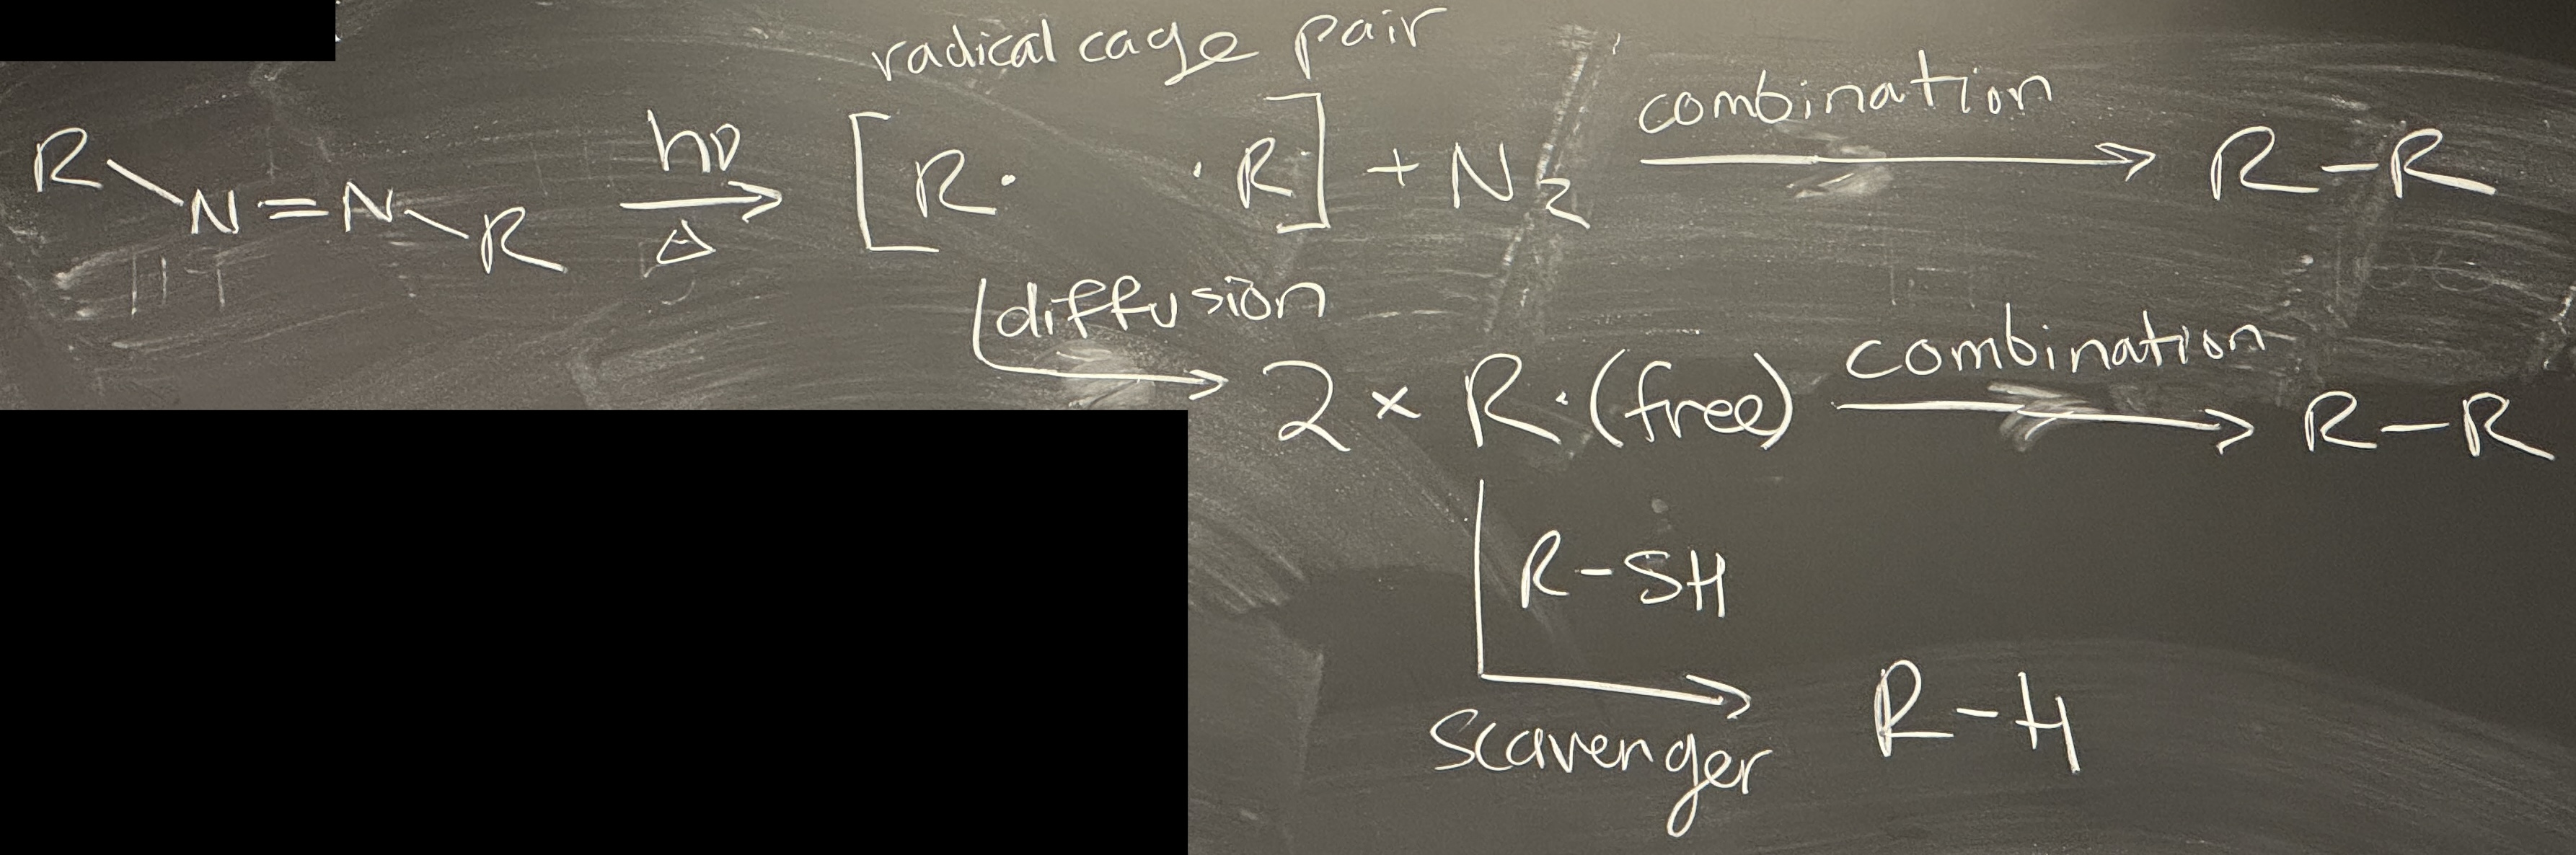
\includegraphics[width=0.8\linewidth]{radCage.JPG}
        \caption{Radical cage effect.}
        \label{fig:radCage}
    \end{figure}
    \begin{itemize}
        \item Consider a radical initiator of the form \ce{R-N=N-R}.
        \item When it decomposes --- either thermally or photochemically --- it will form two radicals that are in very close proximity to each other in solution.
        \begin{itemize}
            \item We call these two radicals a \textbf{radical cage pair}, where the "cage" is the surrounding solvent molecules.
        \end{itemize}
        \item These radicals can easily recombine within the cage in a radical coupling/dimerization reaction to form \ce{R-R}.
        \item However, they can also diffuse out of the cage, drifting apart to yield 2 \ce{R*} in solution.
        \begin{itemize}
            \item These "free" radicals can then combine again to form \ce{R-R}.
            \item Or, alternatively, they can interact with a radical scavenger (such as a thiol\footnote{Alison Wendlandt uses thiols (such as adamantane thiol, \ce{AdSH}) as HAD sources in her research!}) in solution.
        \end{itemize}
        \item Notes on the cage effect.
        \begin{itemize}
            \item A more viscous solvent makes it harder to escape the cage.
            \item A scavenger can differentiate pathways.
            \item Stereoretentive radical reactions can occur within a radical cage, because combination within the cage can outcompete stereoinversion.
            \begin{itemize}
                \item However, if you diffuse out of the cage, forget it.
                \item Takeaway: Cages can have stereochemical consequences, such as retention.
            \end{itemize}
        \end{itemize}
        \item I need to do more reading on this and figure out exactly what I'm responsible for here!!
    \end{itemize}
    \item Radical anions and cations.
    \begin{figure}[h!]
        \centering
        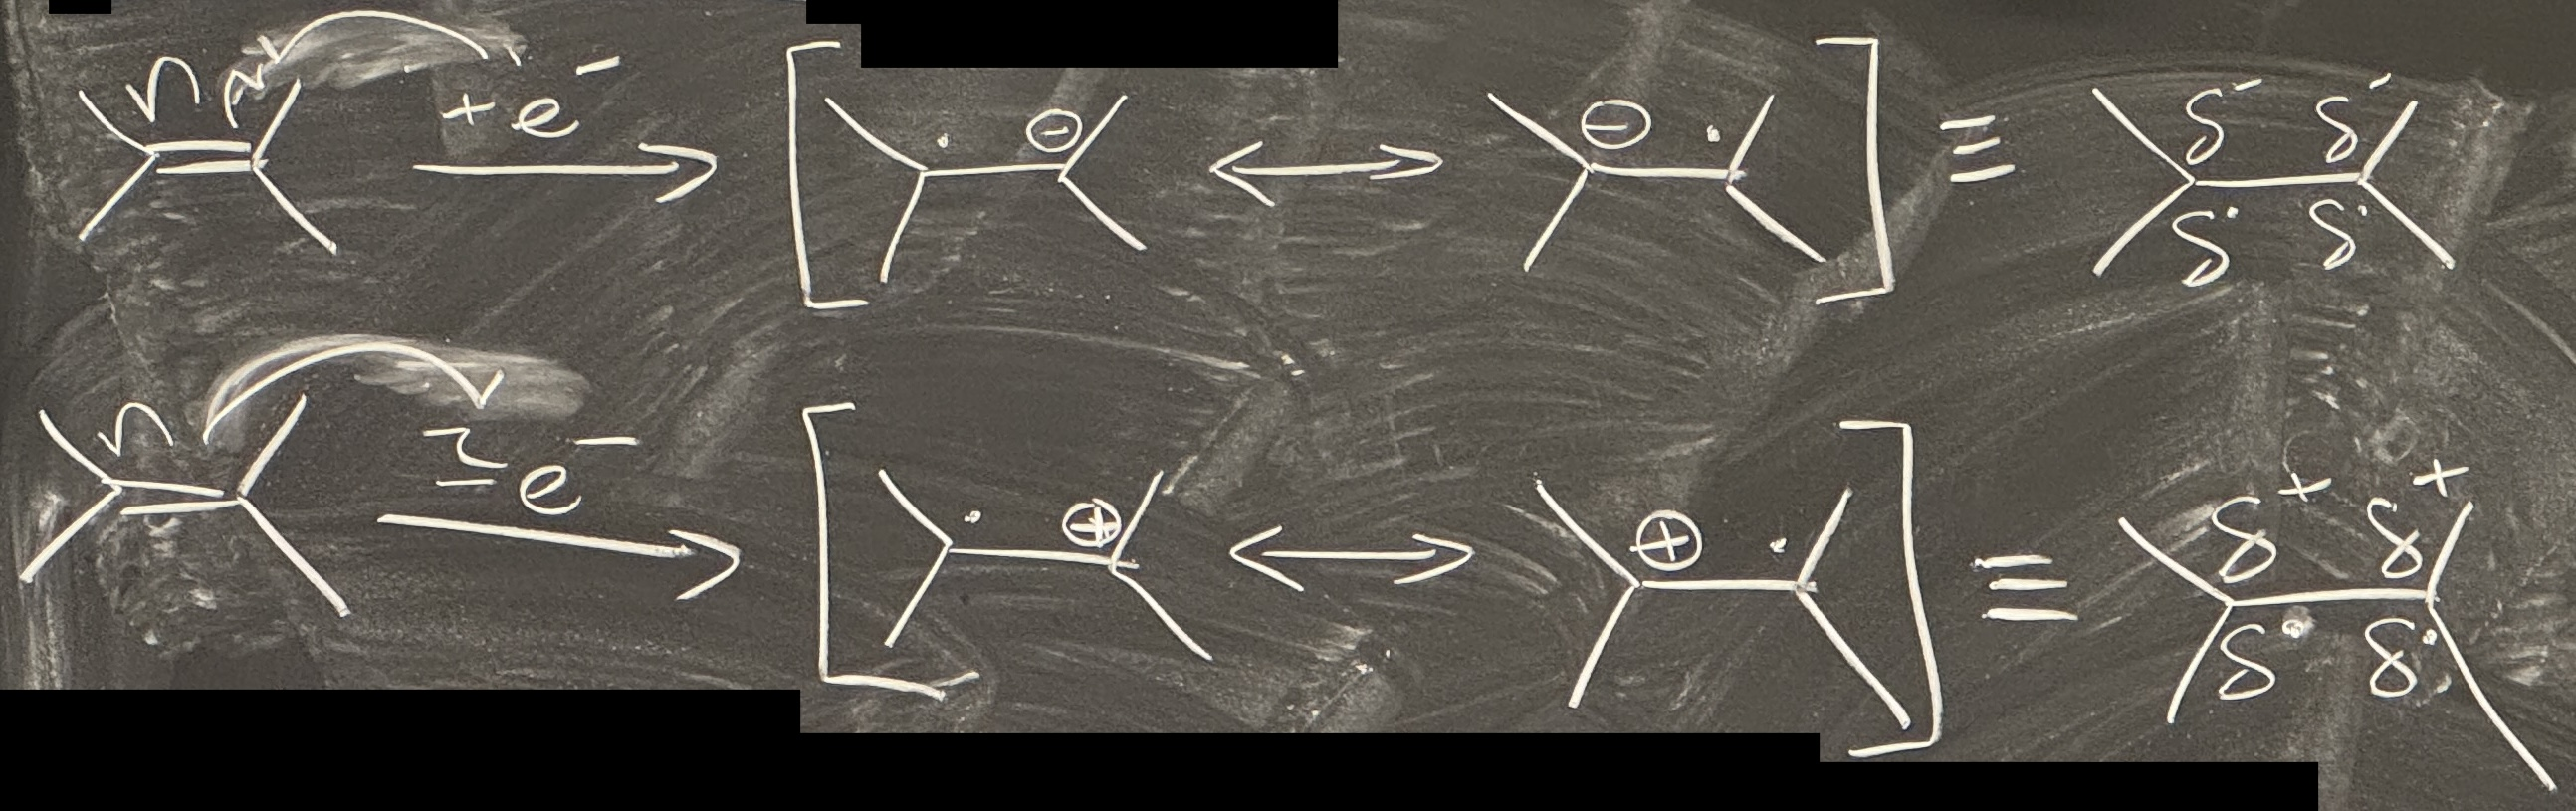
\includegraphics[width=0.7\linewidth]{radIon.JPG}
        \caption{Radical ion formation and structure.}
        \label{fig:radIon}
    \end{figure}
    \begin{itemize}
        \item Start with a $\pi$-system.
        \item When we add an electron to the $\pi$-system or subtract one from it, we form a radical ion.
        \item These radical ions exist in resonance with each other, giving us partial radical and ion character at both sides of the $\pi$-system.
        \item Example of radical cations: Mass spec.
    \end{itemize}
    \item Radical ions are common in aromatic rings.
    \begin{figure}[h!]
        \centering
        \footnotesize
        \begin{subfigure}[b]{0.2\linewidth}
            \centering
            \chemfig{**6(------)}
            \chemmove{
                \node at (cyclecenter1) {$-\cdot$};
            }
            \caption{Radical anion.}
            \label{fig:radIonArNota}
        \end{subfigure}
        \begin{subfigure}[b]{0.2\linewidth}
            \centering
            \chemfig{**6(------)}
            \chemmove{
                \node at (cyclecenter1) {$+\cdot$};
            }
            \caption{Radical cation.}
            \label{fig:radIonArNotb}
        \end{subfigure}
        \begin{subfigure}[b]{0.2\linewidth}
            \centering
            \chemfig{*6(=-=@{C}-=-)}
            \chemmove{
                \node [above right] at (C.center) {$\rceil\rca$};
            }
            \caption{Brackets.}
            \label{fig:radIonArNotc}
        \end{subfigure}
        \caption{Aromatic radical ion notation.}
        \label{fig:radIonArNot}
    \end{figure}
    \pagebreak
    \begin{itemize}
        \item As such, we have a special notation for them.
        \begin{itemize}
            \item Use a circle for the $\pi$-system, and then write "$\pm\cdot$" in the center.
            \item Alternatively, we can write the "$\pm$" and "$\cdot$" on top of each other outside a bracket surrounding the species.
        \end{itemize}
        \item Example of aromatic radical anions: The Birch reduction. See \textcite{bib:CHEM22100Notes}.
    \end{itemize}
    \item Radical ions can undergo \textbf{mesolytic cleavage} to generate a radical plus an ion.
    \begin{equation*}
        \ce{R-X${}^\rceil\rca$ -> R* + X^{$\pm$}}
    \end{equation*}
    \begin{itemize}
        \item This is what happens in mass spec!
        \item It's actually a common phenomenon, even though we often don't think of it in that much detail.
    \end{itemize}
    \item Example of radical ions: A plug for using these species in catalysis.
    \begin{figure}[h!]
        \centering
        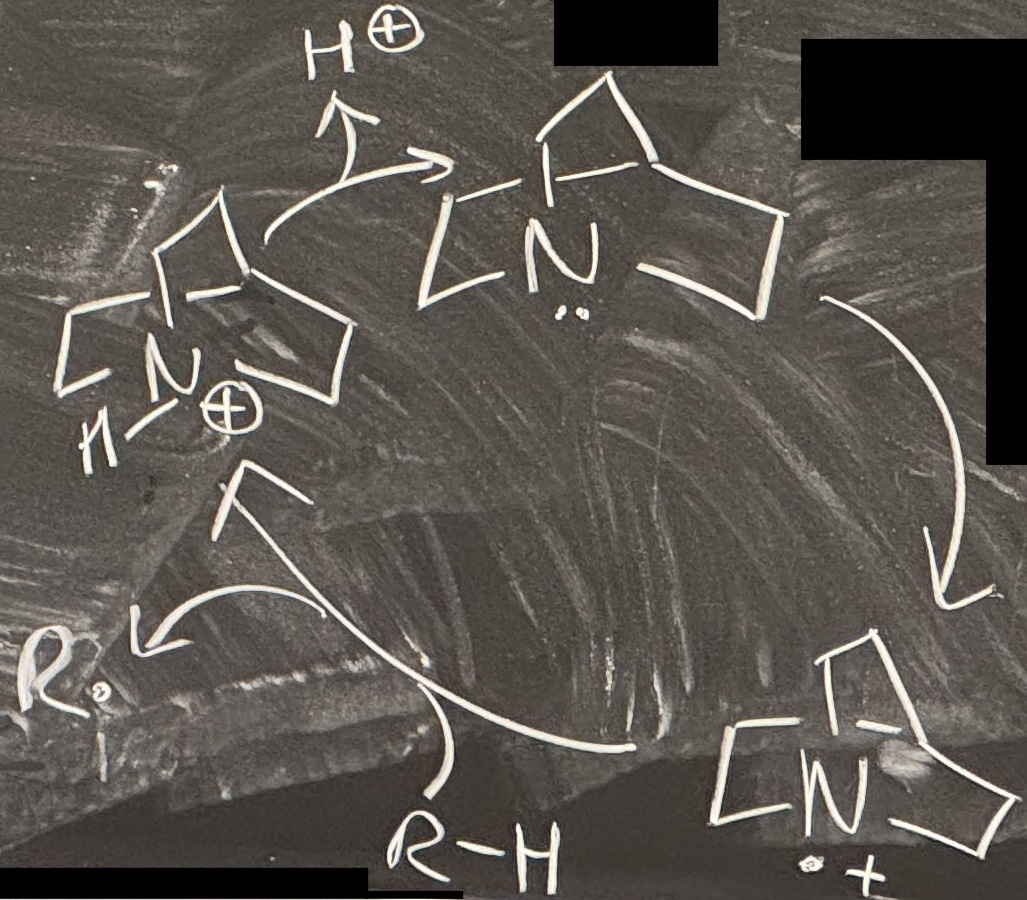
\includegraphics[width=0.27\linewidth]{radIonCat.JPG}
        \caption{Catalysis with radical ions.}
        \label{fig:radIonCat}
    \end{figure}
    \begin{itemize}
        \item Quinuclidine forms a radical cation, reacts with \ce{R-H} to form \ce{R*} and quinuclidinium via an H-atom abstraction (HAA) pathway, and then can reform quinuclidine by loss of a proton. The \ce{R*} then goes on to do cool stuff.
        \item Here, quinuclidine is used as a catalytic initiator!
        \item Reference: \textcite{bib:radIonCat}.
    \end{itemize}
\end{itemize}




\end{document}